\documentclass[conference]{IEEEtran}
\IEEEoverridecommandlockouts
% The preceding line is only needed to identify funding in the first footnote. If that is unneeded, please comment it out.
\usepackage{cite}
\usepackage{amsmath,amssymb,amsfonts}
\usepackage{algorithmic}
\usepackage{graphicx}
\usepackage{textcomp}
\usepackage{xcolor}
\def\BibTeX{{\rm B\kern-.05em{\sc i\kern-.025em b}\kern-.08em
    T\kern-.1667em\lower.7ex\hbox{E}\kern-.125emX}}
\begin{document}

\title{FPGA Acceleration of CNN\\
{\footnotesize \textsuperscript{*}Note: Sub-titles are not captured in Xplore and
should not be used}
\thanks{Identify applicable funding agency here. If none, delete this.}
}

\author{\IEEEauthorblockN{1\textsuperscript{st} Given Name Surname}
\IEEEauthorblockA{\textit{dept. name of organization (of Aff.)} \\
\textit{name of organization (of Aff.)}\\
City, Country \\
email address}
\and
\IEEEauthorblockN{2\textsuperscript{nd} Given Name Surname}
\IEEEauthorblockA{\textit{dept. name of organization (of Aff.)} \\
\textit{name of organization (of Aff.)}\\
City, Country \\
email address}
\and
\IEEEauthorblockN{3\textsuperscript{rd} Given Name Surname}
\IEEEauthorblockA{\textit{dept. name of organization (of Aff.)} \\
\textit{name of organization (of Aff.)}\\
City, Country \\
email address}
}

\maketitle

\begin{abstract}
Let's make CNNs fast
\end{abstract}

\begin{IEEEkeywords}
CNN, FPGA, and more
\end{IEEEkeywords}

\section{Introduction}
With the success of CNNs for various image processing tasks, 3D CNNs have gained attention in video processing. Owing the computational intensity of these CNNs and the power efficiency of FPGA accelerators, recent attention has been on building architectures to leverage FPGAs to accelerate 2D and 3D CNNs. However 3D CNNs  (1) are computationally more intensive than the already intensive 2D CNN (2) consume a lot on on-chip memory if a typical 2D CNN accelerator is used to accelerate 3D CNN. With an added dimension, the design space is also vast and so we will try our best to present a framework which performs design space exploration and chooses the (1) global configurations for the accelerator which will be applied to all the layers and which are needed during compile time, (2) local configurations for each layer which are optimal for that particular layer and which can be presented as instructions to all the accelerator modules at the start of execution of every layer. 

\section{Architecture Design}

Rough draft:
\newline
MemRead reads data and sends to PE0, which is sent to PE1 etc. Good floor design. High frequency. Each PE has a weight buffer, MemReadweight reads from DDR and transfers to every PE through channels. The outputs are transferred to the next PE which appends it output and relays it to next PE etc. 2D arrangement can help reduce the output channels.

The number of PEs is determined by the total DSP blocks available in the target FPGA. It need not necessarily be a divisor of 

Parameter description:
Input - H x W x C x F
Weight - R x S x C x T x K


\section{Optimizations}


\subsection{Convolution layer splitting}\label{AA}
For certain layers where the entire weight does not fit inside the PE weight buffer, the convolution layer (and also the weight) is split into as many sub-layers as needed so that every sub-layer’s weight fits completely inside the PE weight buffer. When C is the number of input channels and weight channels, and if weight does not fit in the on-chip memory of size WBS, then the convolution layer is split into sub-layers each with $C_{sub}$ = WEIGHT\_BUF\_SIZE/(H*W*T) number of channels and the number of sub-layers will be C/$C_{sub}$. Each of these sub-layers will produce output with the same dimension as the original convolution layer. The updated new dimension of input is H x W x $C_{sub}$ x F, weight is R x S x $C_{sub}$ x T x K. (C / $C_{sub}$) -1 sum layers will be needed to accumulate the output results of all the sub-layers to one output. Sum layer takes two volumes of data with the same dimension as the input and accumulates the corresponding elements to produce an output with the same dimensions. Since the volume of output is large and might not fit in the on-chip memory for most of the layers, we need to store the output of every convolution sub-layer to DDR before applying sum layer to them. However, each sum layer can be overlapped with the successive convolution sub-layer - basically sum layer and the following convolution sub-layer will be contending for DDR read and write - but since 3D CNNs are not memory bound, layer splitting and summing shouldn’t have much overhead compared with the normal approach where entire weight fits inside PE.

Why split along channel dimension?: The amount of data read from DDR will be the same as usual convolution layer without splitting. The first set of $C_{sub}$ channels of data and weight will be read for the first sub-layer, second set of Csub channels for the second sub-layer and so on. If the weights are split along T dimension, we have to access the data sub-layer number of times more than normal approach.

\subsection{Tiling}\label{AA}
Compared with 2D CNN, 3D CNNs provide opportunity to reuse data in one more dimension. The input, which resides in global memory and which won’t fit completely in the on-chip memory, will be considered to be made of smaller tiles which entirely fits inside the on-chip data buffer. In the PipeCNN based 3D CNN accelerator, there was up to 10\% reduction in execution time on applying optimal tile size. Optimal tiling ensures that memory operation is not the bottleneck.

Tile dimensions are different for every layer and are calculated based on the size of on-chip data buffer, and amount of data reuse. Two tile dimensions, though consuming same space might have different amount of data reuse. For ex. (let’s ignore channels and) assume a tile of size 3x3x3 (w x h x t) and weight dimension is 3x3x3. This tile produces only one output. While a tile 3x4x4 occupies only 48 bytes it produces 4 outputs while a tile 3x6x3 occupies 54 bytes and produces 4 bytes. The following iteration can find the optimal tile size
\newline
\newline
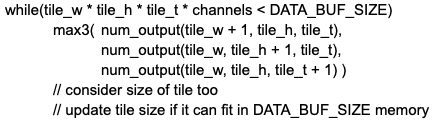
\includegraphics[width=0.5\textwidth]{tiling_snippet}
\newline
\newline
Where num\_output returns the number of outputs that can be produced using the tile size passed to it as parameters and max3 is maximum of 3 numbers. 

\subsection{Data read order}\label{AA}

\end{document}
